%%%%%%%%%%%%%%%%%%%%%%%%%%%%%%%%%%%%%%%%%
% Beamer Presentation
% LaTeX Template
% Version 1.0 (10/11/12)
%
% This template has been downloaded from:
% http://www.LaTeXTemplates.com
%
% License:
% CC BY-NC-SA 3.0 (http://creativecommons.org/licenses/by-nc-sa/3.0/)
%
%%%%%%%%%%%%%%%%%%%%%%%%%%%%%%%%%%%%%%%%%

%----------------------------------------------------------------------------------------
%	PACKAGES AND THEMES
%----------------------------------------------------------------------------------------

\documentclass{beamer}

\mode<presentation> {

% The Beamer class comes with a number of default slide themes
% which change the colors and layouts of slides. Below this is a list
% of all the themes, uncomment each in turn to see what they look like.

%\usetheme{default}
%\usetheme{AnnArbor}
%\usetheme{Antibes}
%\usetheme{Bergen}
%\usetheme{Berkeley}
%\usetheme{Berlin}
%\usetheme{Boadilla}
%\usetheme{CambridgeUS}
%\usetheme{Copenhagen}
%\usetheme{Darmstadt}
%\usetheme{Dresden}
%\usetheme{Frankfurt}
%\usetheme{Goettingen}
%\usetheme{Hannover}
%\usetheme{Ilmenau}
%\usetheme{JuanLesPins}
%\usetheme{Luebeck}
\usetheme{Madrid}
%\usetheme{Malmoe}
%\usetheme{Marburg}
%\usetheme{Montpellier}
%\usetheme{PaloAlto}
%\usetheme{Pittsburgh}
%\usetheme{Rochester}
%\usetheme{Singapore}
%\usetheme{Szeged}
%\usetheme{Warsaw}

% As well as themes, the Beamer class has a number of color themes
% for any slide theme. Uncomment each of these in turn to see how it
% changes the colors of your current slide theme.

%\usecolortheme{albatross}
%\usecolortheme{beaver}
%\usecolortheme{beetle}
%\usecolortheme{crane}
%\usecolortheme{dolphin}
%\usecolortheme{dove}
%\usecolortheme{fly}
%\usecolortheme{lily}
%\usecolortheme{orchid}
%\usecolortheme{rose}
%\usecolortheme{seagull}
%\usecolortheme{seahorse}
%\usecolortheme{whale}
%\usecolortheme{wolverine}

%\setbeamertemplate{footline} % To remove the footer line in all slides uncomment this line
%\setbeamertemplate{footline}[page number] % To replace the footer line in all slides with a simple slide count uncomment this line

%\setbeamertemplate{navigation symbols}{} % To remove the navigation symbols from the bottom of all slides uncomment this line
}

\usepackage{graphicx} % Allows including images
\usepackage{booktabs} % Allows the use of \toprule, \midrule and \bottomrule in tables
\usepackage[absolute,overlay]{textpos}
\setbeamercolor{framesource}{fg=gray}
\setbeamerfont{framesource}{size=\tiny}
\newcommand{\source}[1]{
\begin{textblock*}{6cm}(0.1cm,8.7cm)
    \begin{beamercolorbox}[ht=0.5cm,left]{framesource}
        \usebeamerfont{framesource}\usebeamercolor[fg]{framesource} Image Source: {#1}
    \end{beamercolorbox}
\end{textblock*}}
%----------------------------------------------------------------------------------------
%	TITLE PAGE
%----------------------------------------------------------------------------------------

\title[mvcnn for passange challenge]{Kaggle Passanger Challenge using mvcnn \& LSTM} % The short title appears at the bottom of every slide, the full title is only on the title page

\author{Yuyang Rong} % Your name
\institute[Shanghaitech University] 
% Your institution as it will appear on the bottom of every slide, may be shorthand to save space
{
School of Information Science and Technology \\
Shanghaitech University \\ % Your institution for the title page
\medskip
\textit{rongyy@shanghaitech.edu.cn} % Your email address
}
\date{\today} % Date, can be changed to a custom date

\begin{document}

\begin{frame}
\titlepage % Print the title page as the first slide
\end{frame}

\begin{frame}
\frametitle{Overview} % Table of contents slide, comment this block out to remove it
\tableofcontents % Throughout your presentation, if you choose to use \section{} and \subsection{} commands, these will automatically be printed on this slide as an overview of your presentation
\end{frame}

%----------------------------------------------------------------------------------------
%	PRESENTATION SLIDES
%----------------------------------------------------------------------------------------

%------------------------------------------------
\section{Introduction} % Sections can be created in order to organize your presentation into discrete blocks, all sections and subsections are automatically printed in the table of contents as an overview of the talk
%------------------------------------------------

\begin{frame}
\frametitle{Motivation}
	\begin{itemize}
	\item Is any passenger carrying dangerous objects? 
	\item Transportation Security Administration(TSA): Use Millimeter Wave Unit to find out
	\item The image can be vague and unclear.
	\item Humans is not efficient in determining whether a passenger is carrying banned object.
	\item \textbf{How can machines help?}
	\end{itemize}
	\begin{figure}
		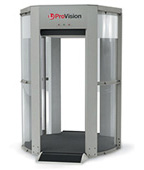
\includegraphics[width=2cm]{../Pic/MillimeterWaveUnit.jpg}
		\caption{Millimeter Wave Unit}
	\end{figure}
	\source{https://en.wikipedia.org/wiki/Millimeter\_wave\_scanner}
\end{frame}

%------------------------------------------------
\section{Problem Statement} % Sections can be created in order to organize your presentation into discrete blocks, all sections and subsections are automatically printed in the table of contents as an overview of the talk
%------------------------------------------------

%------------------------------------------------
\begin{frame}
\frametitle{Problem Statement}
	\begin{itemize}
	\item Let's talk about humans first.
	\item Even if someone is carrying forbidden objects, how to tell where it is?
	\item We define 17 regions out of human body.
	\end{itemize}
	\begin{figure}
		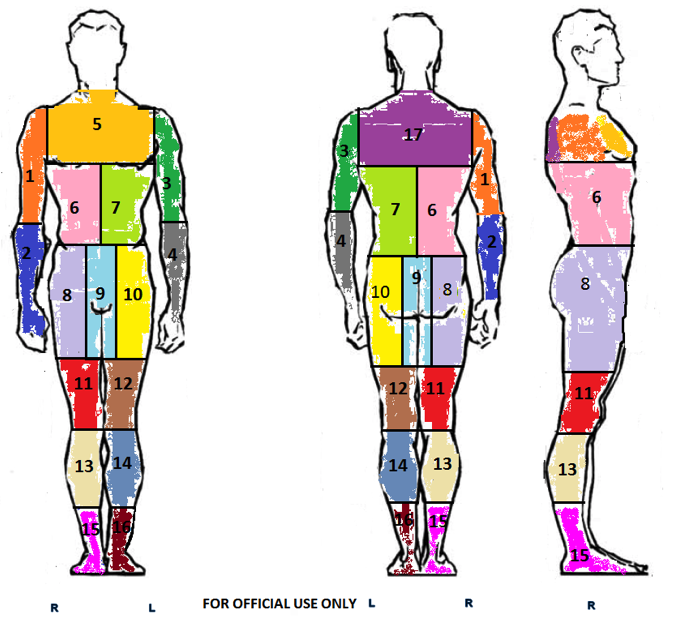
\includegraphics[width=6cm]{../Pic/body_zones.png}
		\caption{Region Definition}
	\end{figure}
	\source{TSA: Definition}
\end{frame}
%------------------------------------------------
\begin{frame}
\frametitle{Problem Statement}
	\begin{itemize}
		\item Given a consecutive images of one person from 16 different angles with labels of 17 regions.
		\item Train a network to predict if there is dangerous object for each of 17 regions.
	\end{itemize}
\end{frame}
%------------------------------------------------

\begin{frame}
\frametitle{Problem Statement}
	\begin{figure}
		\centering
		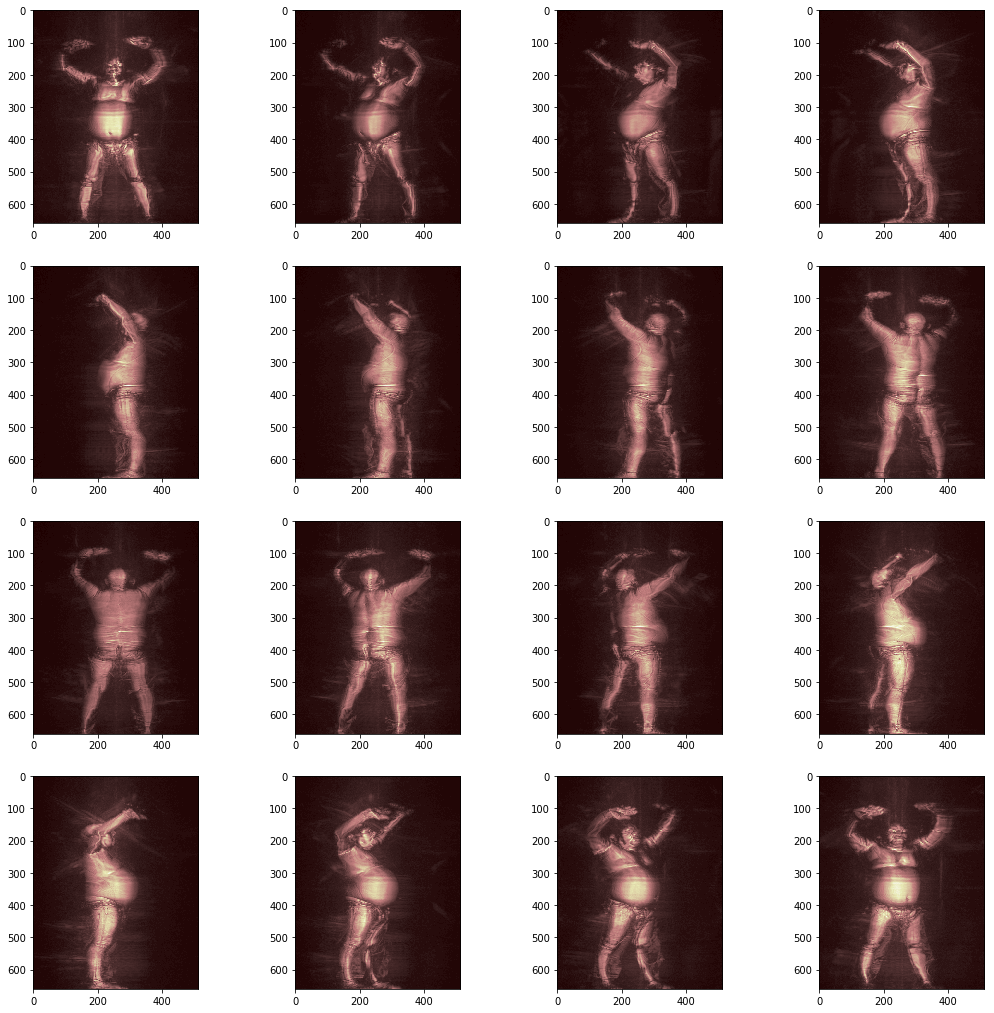
\includegraphics[width=6cm]{../Pic/ffefec0cd4e1e2c3fe64bb93f082efdd.png}
		\caption{Region Definition}
	\end{figure}	
	\source{TSA: Dataset}
\end{frame}

%------------------------------------------------

\section{Difficulties}
\begin{frame}
\frametitle{Difficulties}
	\begin{itemize}
		\item No or little feature and Noise, even human cannot label it well.
		\item Broken and rigged data: Not all regions are labeled.
		\item Not much positive labels. Of 1k people and 10k labels, only about 1k positive labels
		\item The file is too big. Low resolution images(listed above) takes 10M per person.
	\end{itemize}
\end{frame}

\begin{frame}
\frametitle{Difficulties: Noisy Data}
	\begin{figure}
		\centering
		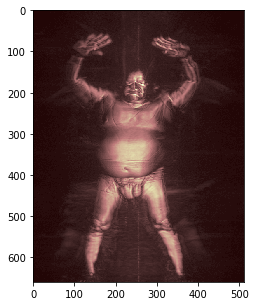
\includegraphics[width=6cm]{../Pic/noisy.png}
		\caption{This person is labeled to have dangerous objects in his right arm and crotch}
	\end{figure}	
	\source{TSA: Dataset}
\end{frame}

\begin{frame}
\frametitle{Difficulties: Rigged Data}
	\begin{figure}
		\centering
		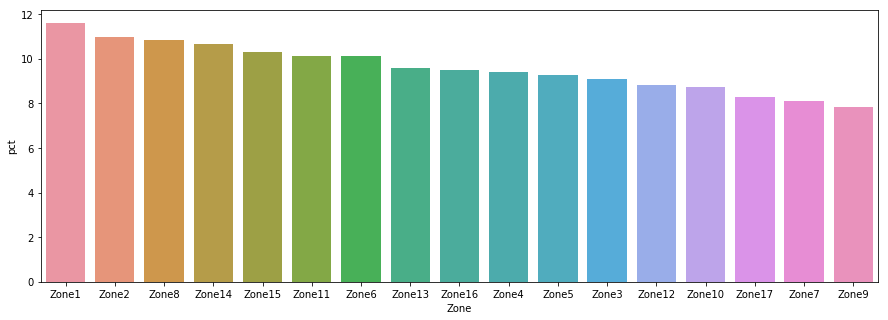
\includegraphics[width=10cm]{../Pic/bars.png}
		\caption{The most popular to hide things is your right arm and the least popular one is crotch?}
	\end{figure}	
\end{frame}


%------------------------------------------------
\section{Out Approach} % Sections can be created in order to organize your presentation into discrete blocks, all sections and subsections are automatically printed in the table of contents as an overview of the talk
%------------------------------------------------

%------------------------------------------------
\begin{frame}
\frametitle{Our Approach: Crop \& PCA}

	

\end{frame}

%------------------------------------------------
\begin{frame}
\frametitle{Multi-view CNN}

	

\end{frame}

%------------------------------------------------
\begin{frame}
\frametitle{Our Approach: mvcnn with attention}

	

\end{frame}

%------------------------------------------------
\begin{frame}
\frametitle{Our Approach: mvcnn with LSTM attention}

	

\end{frame}

%------------------------------------------------
\begin{frame}
\frametitle{SGDR Optimization}

	

\end{frame}

%------------------------------------------------
\begin{frame}
\frametitle{Our Approach: Filling Channel with Avg \& Std (Experimenting)}

	

\end{frame}


%------------------------------------------------
\section{Experiment} % Sections can be created in order to organize your presentation into discrete blocks, all sections and subsections are automatically printed in the table of contents as an overview of the talk
%------------------------------------------------

%------------------------------------------------
\begin{frame}
\frametitle{Experiment Result}

	

\end{frame}

\end{document} 